\documentclass[a4paper, oneside, 12pt]{book}
%\documentclass[12pt]{article}
\usepackage[spanish, english, es-tabla]{babel}
\usepackage[utf8]{inputenc}
\usepackage[left = 2cm, right = 2cm, bottom = 2cm, top = 3cm]{geometry}
\usepackage{amsmath, amssymb}
\usepackage{graphicx}
\usepackage{hyperref}
\usepackage{listings}
\usepackage{courier}

\usepackage[dvipsnames]{xcolor}

% Portada Oficial
\usepackage[export]{adjustbox}

\renewcommand{\lstlistingname}{Ejemplo}
\renewcommand{\lstlistlistingname}{Listado de ejemplos}

% https://tex.stackexchange.com/questions/60209/how-to-add-an-extra-level-of-sections-with-headings-below-subsubsection
%\newcommand{\subsubsubsection}[1]{\paragraph{#1}\mbox{}\\}
%\setcounter{secnumdepth}{4}
%\setcounter{tocdepth}{4}

% Configuracion PDF metadata
\hypersetup{
	pdftitle= {Diseño y desarrollo de un microservicio para la monitorización y precicción de tráfico en red},
	pdfauthor = {Enrique Fernández Sánchez},
	pdfsubject = {Gestión de datos de monitorización y predicción de tráfico en red},
	pdfkeywords = {Microservicio, Monitorización, Predicción, Python, FastAPI, Network Forecast}
}

% Configuracion colores hiperenlaces
\hypersetup{
	colorlinks=true,
	linkcolor=black,
	%filecolor=magenta,      
	urlcolor=cyan,
}

% Configure lstlisting
\definecolor{codegreen}{rgb}{0,0.6,0}
\definecolor{codegray}{rgb}{0.5,0.5,0.5}
\definecolor{codepurple}{rgb}{0.58,0,0.82}
\definecolor{backcolour}{rgb}{0.95,0.95,0.92}

\lstdefinestyle{mystyle}{
	backgroundcolor=\color{backcolour},   
	commentstyle=\color{codegreen},
	keywordstyle=\color{magenta},
	numberstyle=\tiny\color{codegray},
	stringstyle=\color{codepurple},
	basicstyle=\ttfamily\footnotesize,
	breakatwhitespace=false,         
	breaklines=true,                 
	captionpos=t,                    
	keepspaces=true,                 
	numbers=left,                    
	numbersep=5pt,                  
	showspaces=false,                
	showstringspaces=false,
	showtabs=false,                  
	tabsize=2
}

\lstset{style=mystyle}

% Configuracion encabezados y pies de pagina
\usepackage{fancyhdr}
\fancyhf{}
\lhead[\leftmark]{\small TFM: Enrique Fernández Sánchez}
\rhead[Nombre Autor]{\rightmark}
\cfoot[\thepage]{}
\cfoot[]{\thepage}
\renewcommand{\headrulewidth}{0.5pt}
\renewcommand{\footrulewidth}{0pt}
\fancypagestyle{plain}{
	\fancyhf{}
	\fancyhead[L]{\small TFM: Enrique Fernández Sánchez}
	\fancyfoot[C]{\thepage}
	%\renewcommand{\headrulewidth}{0pt}		% Sirve para eliminar linea
	%\renewcommand{\footrulewidth}{0pt}		% Sirve para eliminar linea
}
\pagestyle{fancy}

\begin{document}
	\selectlanguage{spanish}
	
	%% PORTADA UPCT
	\thispagestyle{empty}
	
	\newgeometry{left=0.01cm, bottom=0.01cm, top=0.01cm}
	
	\begin{minipage}{0.2\textwidth}
		
\includegraphics[height=\textheight, left]{img/banda_etsit_90.png}
	\end{minipage}
	\centerline{\begin{minipage}[t][6cm][b]{0.5\textwidth}
			\title{\textbf{Diseño y desarrollo de un microservicio para la gestión de información de monitorización y predicciones de tráfico en red}} 
			
			%\date{1 enero 2023}
			
			\maketitle
			
			\vspace{0.5cm}
			\hspace{1.5cm} \textbf{TRABAJO FIN DE MÁSTER} \\
			
			\vspace{0.5cm}
			\hspace{1.15cm} Máster Universitario en Ingeniería de \\   \vspace{-0.5cm}
			\hspace{3cm}Telecomunicación \\
			
			\vspace{2cm}
			\textbf{Autor:} \author{Enrique Fernández Sánchez} \\
			
			\textbf{Tutor:} Pablo Pavón Mariño
	\end{minipage}}
	
	\restoregeometry
	%% END PORTADA UPCT	
	
	\pagebreak
	
	\tableofcontents
	
	\pagebreak
	
	\addcontentsline{toc}{section}{Índice de figuras}
	\listoffigures
	
	\pagebreak
	
	\addcontentsline{toc}{section}{Listado de ejemplos}
	\lstlistoflistings
	
	\pagebreak
	
	\chapter{Introducción}
	
	\section{Contexto del trabajo}
	
	\section{Motivación}
	
	\section{Descripción Global}
	
	\section{Objetivos}
	
	\section{Resumen capítulos de la memoria}
	
	\pagebreak
	
	\chapter{Tecnologías empleadas}
	
	\noindent En este capítulo, se van a presentar las diferentes tecnologías utilizadas para la implementación de la aplicación.
	
	\section{Arquitectura y microservicios}
	
	\noindent En primer lugar, se va a comentar acerca de la arquitectura escogida. En este caso, se decide realizar una implementación basada en microservicios utilizando una REST API. \\
	
	
	\noindent \textbf{\large Arquitectura basada en \textbf{microservicios}} \\
	
	\noindent Lo primero, es entender en que consiste un microservicio. Para ello, podemos definirlo como los sistemas que cumplen las siguientes premisas: [\ref{bib: microservices}]
	
	\begin{itemize}
		\item Los microservicios son sistemas pequeños, independientes y poco ''acoplados''.
		
		\item Cada servicio tiene su propio código fuente, que esta separado del resto de códigos de los servicios.
		
		\item Cada servicio se puede desplegar de manera independiente. 
		
		\item Cada servicio es responsable de la persistencia de sus datos.
		
		\item Los servicios se comunican entre sí utilizando APIs
		
		\item Además, como ventaja, los servicios no tienen por qué estar implementados todos en el mismo lenguaje de programación.
	\end{itemize}

	\noindent Por lo tanto, dado los objetivos presentados en este trabajo, se llegó a la conclusión de que tratar el sistema propuesto como un microservicio podría aportar numerosas ventajas, ya que permitiría ser utilizado por otros servicios, extendiendo la funcionalidad de estos y añadiendo un valor extra. Para ello, será necesario definir la API que utilizaremos para comunicarnos con el sistema.
	
	\pagebreak
	
	\noindent \textbf{\large Comunicación basada en \textbf{API}} \\
	
	\noindent Una API permite a dos componentes comunicarse entre sí mediante una serie de reglas. Además, supone un ''contrato'' en el que se establecen las solicitudes y respuestas esperadas en la comunicación. [\ref{bib: what is api}] \\
	
	\noindent Dependiendo de la implementación de la API que se realice, distinguimos cuatro tipos de API:
	
	\begin{itemize}
		\item API de SOAP. Utilizan un protocolo de acceso a objetos. Los interlocutores intercambian mensajes XML. En general, es una solución poco flexible.
		
		\item API de RPC. Basado en llamadas de procedimientos remotos. El cliente ejecuta una función en el servidor, y este responde con la salida de la función.
		
		\item API de WebSocket. Solución moderna de desarrollo de API, que utiliza objetos JSON y un canal bidireccional para realizar la comunicación entre el cliente y el servidor.
		
		\item API de REST. Solución más popular. El cliente envía solicitudes al servidor como datos, utilizando métodos HTTP. Es una opción muy flexible.
	\end{itemize}
	
	\noindent En en caso de nuestra aplicación, se decidió utilizar el tipo REST API, ya que permite una sencilla implementación de cara al cliente que quiera utilizar dicha interfaz.
	
	
	\pagebreak
	
	\section{Bases de datos}
	
	\noindent Para asegurar la persistencia de los datos en nuestra aplicación, es necesario utilizar una base de datos. En dicha base de datos, guardaremos información relevante para el correcto funcionamiento del sistema, en nuestro caso, redes y/o interfaces a monitorizar, o los datos monitorizados. \\
	
	\noindent En la aplicación de monitorización, distinguimos entre datos de dos tipos:
	
	\begin{itemize}
		\item Datos clásicos. Como por ejemplo, la información asociada a una red a monitorizar.
		\item Datos de tipo ''time series''. Como por ejemplo, las muestras de monitorización de una red.
	\end{itemize}

	\noindent En primer lugar, se diseña una base de datos tipo SQL para almacenar los ''datos clásicos''. Y por otro lado, se diseña una base de datos diferente, especializada para el almacenamiento de datos tipo ''time series'', en este caso, se elige una base de datos llamada InfluxDB.
	
	\subsection{Base de datos tipo relacional/SQL}
	
	\noindent SQL es una base de datos de tipo relacional. Dichas bases de datos, suponen una colección de información que organizan los datos en una serie de ''relaciones'' cuando la información es almacenada en una o varias ''tablas''. Por lo tanto, las relaciones suponen conexiones entre diferentes tablas, permitiendo así una asociación entre información diferente. [\ref{bib: relational database}] \\
	
	\noindent Por ejemplo, si vemos la figura \ref{img: example sql}, podemos comprobar como se realizan las relaciones entre las diferentes tablas (Ratings, Users, Movies o Tags), se realiza mediante uno de los campos definidos en la propia tabla. Por ejemplo, el campo ''user\_id'' de la tabla Ratings, permite una relación con la tabla Users, con el campo ''id''.
	
	\begin{figure}[h!]
		\begin{center}
			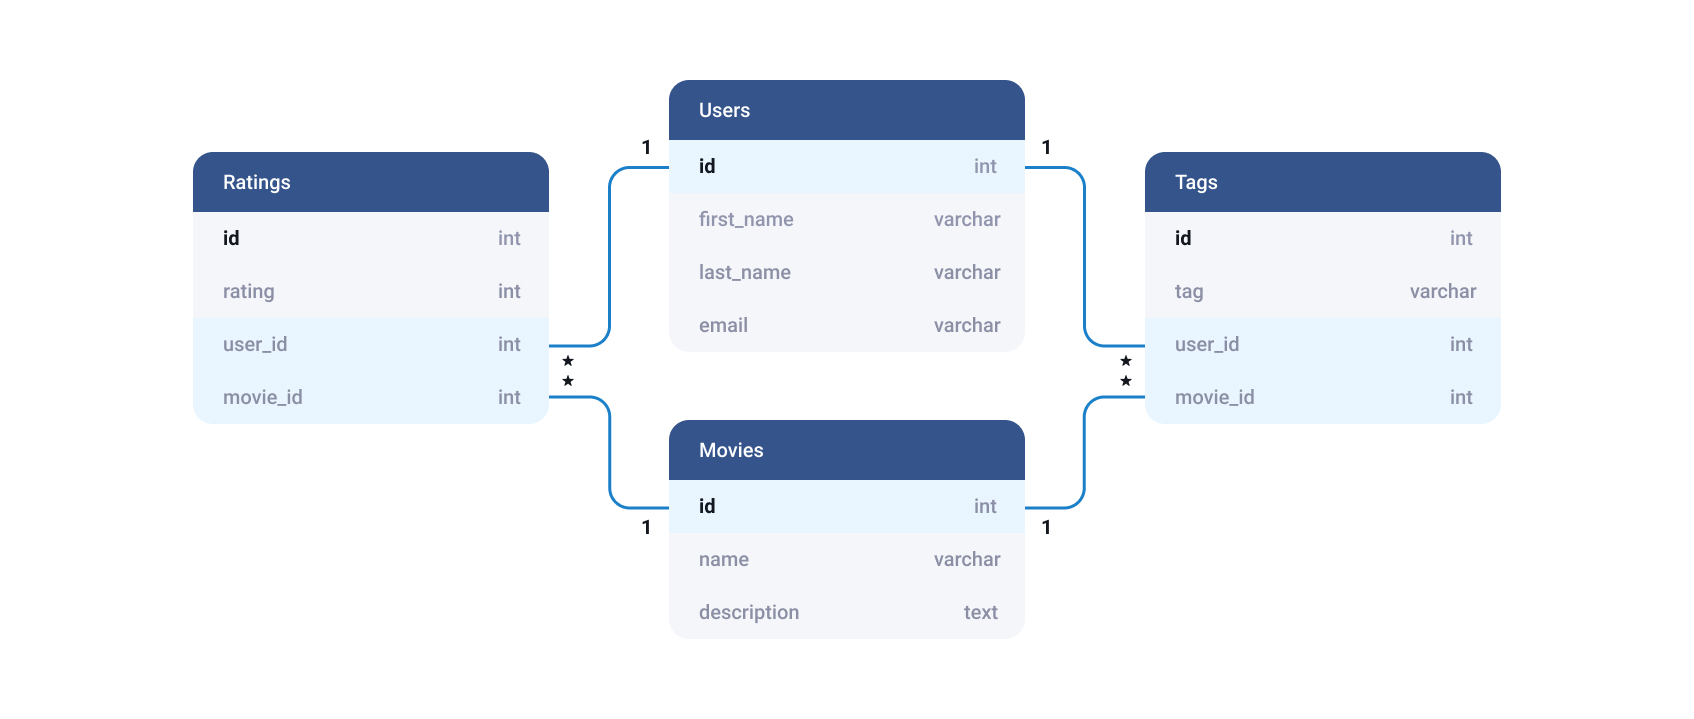
\includegraphics[width=0.95\textwidth]{img/example_relational_database.jpg}
			\caption{Ejemplo de relaciones dentro de una base de datos SQL. [\ref{bib_img: example sql}]}
			\label{img: example sql}
		\end{center}
	\end{figure}
	
	\noindent Para el caso de nuestra aplicación de monitorización de tráfico en red, modelamos la base de datos según la información que vamos a almacenar. Por lo que tenemos que definir la estructura de tablas, los campos que van a tener cada una de las tablas, y los campos por los que se van a relacionar entre sí. A esta información la llamamos modelo de datos.
	
	\pagebreak
	
	\subsubsection{Modelos de datos}
	
	\noindent El primer modelo de datos de la aplicación, es el referido a la información de una red a monitorizar. La descripción del modelo la podemos ver en la figura \ref{img: modelo sql networks}.
	
	\begin{figure}[h!]
		\begin{center}
			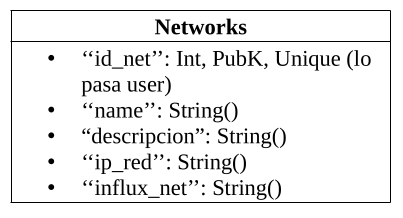
\includegraphics[width=0.5\textwidth]{img/model_sql_networks.png}
			\caption{Modelo de datos para las redes a monitorizar. Equivale con la tabla ''networks''.}
			\label{img: modelo sql networks}
		\end{center}
	\end{figure}
	
	\noindent El segundo modelo de datos de la aplicación, es el referido a la información de una interfaz a monitorizar, que esta dentro de una red monitorizada. La descripción del modelo la podemos ver en la figura \ref{img: modelo sql interfaces}.

	\begin{figure}[h!]
		\begin{center}
			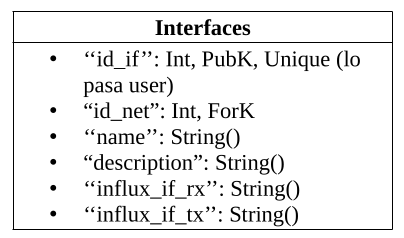
\includegraphics[width=0.5\textwidth]{img/model_sql_interfaces.png}
			\caption{Modelos de datos para las interfaces a monitorizar. Equivale con la tabla ''interfaces''}
			\label{img: modelo sql interfaces}
		\end{center}
	\end{figure}

	\noindent Se establece una relación del modo que una interfaz solo puede pertenecer a una red monitorizada, y que además, una red monitorizada puede tener muchas interfaces. Dicha relación se realiza mediante el campo ''id\_net'' de la tabla Interfaces. \\
	
	\noindent Por último, la base de datos SQL utilizada para esta aplicación es PostgreSQL [\ref{bib: postgresql}], ya que además de ser Open Source, permite una gran escalabilidad, amoldándose a los recursos de la máquina en la que esté funcionando.
	
	\pagebreak
	
	\subsection{Base de datos tipo ``time series''/InfluxDB} 
	
	\noindent InfluxDB es una base de datos diseñada para trabajar con datos tipo time-series. Si bien es cierto que SQL puede gestionar este tipo de datos, no fue creado estrictamente para este objetivo. En este caso, InfluxDB esta diseñado para almacenar grandes volúmenes de datos, y además realizar análisis en tiempo real sobre esos datos. \\
	
	\noindent En comparación con SQL, en InfluxDB un ``timestamp'' identifica un punto en cualquier serie de datos. Esto sería equivalente a SQL, si la clave primaria de una tabla es establecida por el sistema y siempre es equivalente al tiempo. Además, InfluxDB permite reconocer el ``schema'' de manera dinámica, además de que no estas obligado a definir el ``schema'' y seguirlo, es decir, se permiten cambios dentro de la misma serie de datos. [\ref{bib: influxdb doc vs sql}] \\
	
	\noindent Algunas de las razones destacadas para elegir InfluxDB son: [\ref{bib: influxdb doc}]
	
	\begin{itemize}
		\item Perfecto para almacenar datos de telemetría, como métricas de aplicaciones o sensores IoT.
		\item Los datos son comprimidos automáticamente para ser eficientes con el espacio disponible.
		\item Se realizan tareas automáticas de ``downsampling'' para reducir el uso de disco.
		\item Lenguaje para hacer consultas que permite analizar en profundidad los datos almacenados.
		\item Disponible una aplicación web para realizar consultas y comprobar los datos disponibles en la base de datos.
	\end{itemize}

	\vspace{10px}

	\noindent \textbf{\large Terminología} \\
	
	\noindent Comparando con los conceptos ya existentes en bases de datos de tipo SQL, se definen los siguientes conceptos en InfluxDB:
	
	\begin{itemize}
		\item ``measurement'': equivalente a una tabla.
		\item ``tags'': equivalente a columnas indexadas dentro de una tabla.
		\item ``fields'': equivalente a columnas no indexadas dentro de una tabla.
		\item ``points'': similar a las filas en una tabla.
	\end{itemize}

	\vspace{20px}

	\begin{figure}[h!]
		\begin{center}
			
\includegraphics[width=0.6\textwidth]{img/InfluxDB.png}
			\caption{Logotipo base de datos InfluxDB.}
			\label{img: influxdb logo}
		\end{center}
	\end{figure}

	\pagebreak

	\noindent \textbf{\large Modelo de datos} \\
	
	\noindent Para la aplicación a diseñar, se plantea la premisa de que en la base de datos InfluxDB solo se van a guardar los datos de cada muestra de monitorización de una interfaz. Además, se pueden tener tantas redes como sean necesarias, y dentro de cada red, tantas interfaces como creamos necesarias. \\
	
	\noindent En resumen, definimos el modelo de datos que tiene que seguir nuestra aplicación:
	
	\begin{itemize}
		\item ``measurement'': equivalente a una red a monitorizar, valor almacenado en Networks::influx\_net.
		\item ``fields'': nombre del valor a monitorizado, en este caso el default es \textit{link\_count}.
		\item ``tags'': solo tenemos un tag llamado \textit{interface}, su objetivo es identificar a que interfaz pertenece el punto de monitorización. El valor puede estar ser Interfaces::influx\_if\_rx o Interfaces::influx\_if\_tx.
		\item ``points'': corresponde con el valor numérico del ``field''. En este caso, corresponde con el valor númerico de link\_count en ese periodo de 5 minutos.
	\end{itemize} 
	
	
	\pagebreak
	
	\section{Modelo de predicción}
	
	\pagebreak
	
	\section[Lenguajes y frameworks]{Lenguajes de programación y frameworks}
	
	\noindent En resumen, para el desarrollo de esta aplicación se han utilizado el lenguaje de programación Python, con el framework de desarrollo para APIs FastAPI.
	
	\pagebreak
	
	\section[Despliegue en Producción]{Tecnologías utilizadas en un despliegue en producción}
	
	\noindent \textbf{\large Docker} \\
	
	\noindent \textbf{\large docker-compose} \\
	
	\noindent \textbf{\large Traefik} \\
	
	\pagebreak
	
	\chapter{Diseño e implementación del sistema}
	
	\section{Descripción REST API}
	
	\section{Estructura de la aplicación}
	
	\section{Modelos de datos}
	
	\section{Endpoints}
	
	\section{Implementación del sistema}
	
	\pagebreak
	
	\chapter{Pruebas y validación del sistema}
	
	\pagebreak
	
	\chapter{Conclusiones}
	
	\section{Propuestas futuras}
	
	\pagebreak
	
	\chapter{Bibliografía}
	
	\subsection*{Enlaces y referencias}
	\addcontentsline{toc}{section}{Enlaces y referencias}
	
	\begin{enumerate}
		% 1
		\item
		\label{bib: what is api}
		\href{https://aws.amazon.com/es/what-is/api/}{¿Qué es una API?}
		
		% 2
		\item
		\label{bib: microservices}
		\href{https://learn.microsoft.com/en-us/azure/architecture/guide/architecture-styles/microservices}{Microservice architecture style}
		
		
		% 3
		\item
		\label{bib: relational database}
		\href{https://cloud.google.com/learn/what-is-a-relational-database}{What is a relational database?}
		
		
		% 4
		\item
		\label{bib: postgresql}
		\href{https://www.postgresql.org/}{PostgreSQL}
		
		% 5
		\item
		\label{bib: influxdb doc}
		\href{https://www.stackhero.io/en/services/InfluxDB/documentations/Introduction#differences-between-influxdb-and-relational-sql-databases}{InfluxDB: Introduction}
		
		
		% 5
		\item
		\label{bib: influxdb doc vs sql}
		\href{https://archive.docs.influxdata.com/influxdb/v1.2/concepts/crosswalk/}{InfluxDB: Comparison to SQL}
		
	\end{enumerate}

	\vspace{20px}
	
	\subsection*{Figuras}
	\addcontentsline{toc}{section}{Imagenes}

	\begin{enumerate}
		% 1
		\item
		\label{bib_img: example sql}
		\href{https://xbsoftware.com/blog/main-types-of-database-management-systems/}{Relational Databases}
	\end{enumerate}
	
	\pagebreak
	
	\chapter*{Anexos}
	\addcontentsline{toc}{chapter}{Anexos}
	
	\section*{Anexo I. Generación dataset sintético}
	\addcontentsline{toc}{section}{Anexo I. Generación dataset sintético}
	
\end{document}